\documentclass{standalone}

\usepackage{tikz}
    \usetikzlibrary{arrows.meta}
    
\begin{document}
\begin{tikzpicture}
    % \draw[help lines] (0,0) grid (11,5);
    \node at (5,5) {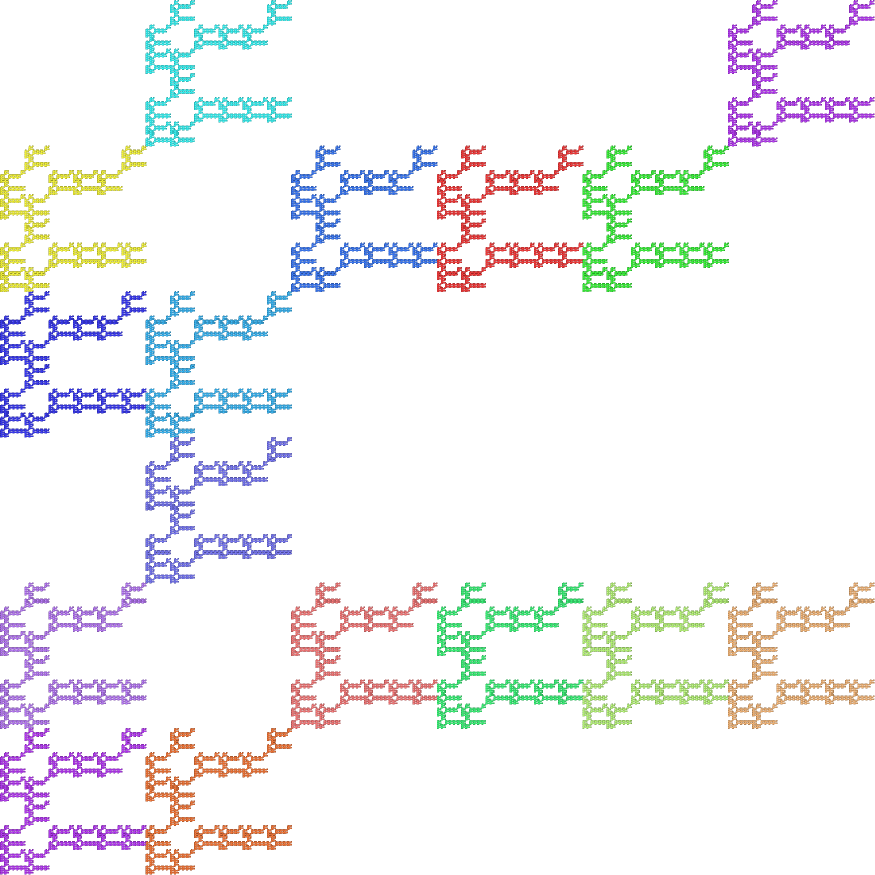
\includegraphics[width=10cm]{D6-type.png}};
    \foreach \x in
        {(0,0), (10,10), (0,2), (10,2), (2,0), (2,10)} 
        {\fill \x circle(0.15);}
    \path[->,>={Latex[length=5mm]}, line width=1mm, red]
        (-0.7,-0.7) edge (0,0)
        (10.7,10.7) edge (10,10);
    \path[->,>={Latex[length=5mm]}, line width=1mm, blue]
        (-1,2) edge (0,2)
        (11,2) edge (10,2);
    \path[->,>={Latex[length=5mm]}, line width=1mm, black]
        (2,-1) edge (2,0)
        (2,11) edge (2,10);
\end{tikzpicture}
\end{document}